\section{Problem Statement}
\label{sec:problemStatement_IS}

%Web browsers and web interfaces are nowadays one of the predominant ways to interact with remote systems.
Many sensitive applications such as e-banking or e-voting, safety-critical systems such as remote industrial PLCs, and medical devices provide web-based interfaces where users input parameters. Typically, devices such as computers and smartphones run complex software, e.g., operating systems and browsers, among other applications, but still, they are used to access sensitive remote services. Hence, these platforms expose a large attack surface from OS level to the JavaScript and browser extensions~\cite{driveByDownload, extensionSecurity, extensionSecurity1, extensionHack1, microsoftPatches, kernelSecurity, linuxMalware, zeusMalware, wannacry}. An attacker-controlled host can modify the user inputs to profit or cause intentional damage to the remote services.

\emph{Trusted path}~\cite{x86} provides a secure channel between the user and a trusted service (usually mediated by a trusted app on the local system). Existing trusted path solutions typically are based on two approaches: i) \textit{trusted execution environments} (TEEs)~\cite{sgxio} which rely on the OS and its drivers to communicate with the IO devices; therefore, they should be combined with a trusted hypervisor, which increases the TCB significantly; and ii) \textit{transaction confirmation devices}~\cite{filyanov2011uni}, which introduce high cognitive load to the users, risk user habituation and are limited to specific use cases.

The goal of this work is to design a system that protects the interaction between the user (who uses a traditional local host) and the remote server without relying on trusted hypervisors, specialized hardware like TEEs, or solutions with high cognitive load to users and that risk habituation such as transaction confirmation devices.

\subsection{System and Adversary Model}
\label{sec:problemStatement:systemMode}

Figure~\ref{integriscreen:fig:systemModel} shows an overview of a visual supervision system: the user owns a local host (i.e., a desktop or laptop computer) and provides sensitive inputs via a web form to a remote server over the network. We assume that both the host and the network are fully compromised, while the remote server is a trusted entity. 
%The remote server requires form-based user inputs, accessible via a web browser running on the host. As such, all the data whose integrity needs to be protected is presented on the host's screen.

The user inputs data via a keyboard or a mouse that is connected to the host system. The user's interaction with the local host is visually supervised by a trusted application running on a device equipped with a camera, e.g., a smartphone, placed such that it can continuously capture the contents of the host screen during input. 
For simplicity, we refer to this device as a smartphone in the rest of this chapter -- however, the proposed technique generalizes to any device with network connectivity and a front-facing camera, such as an augmented reality (AR) headsets or a smart home assistant device.

\begin{figure}[t]
	\centering
    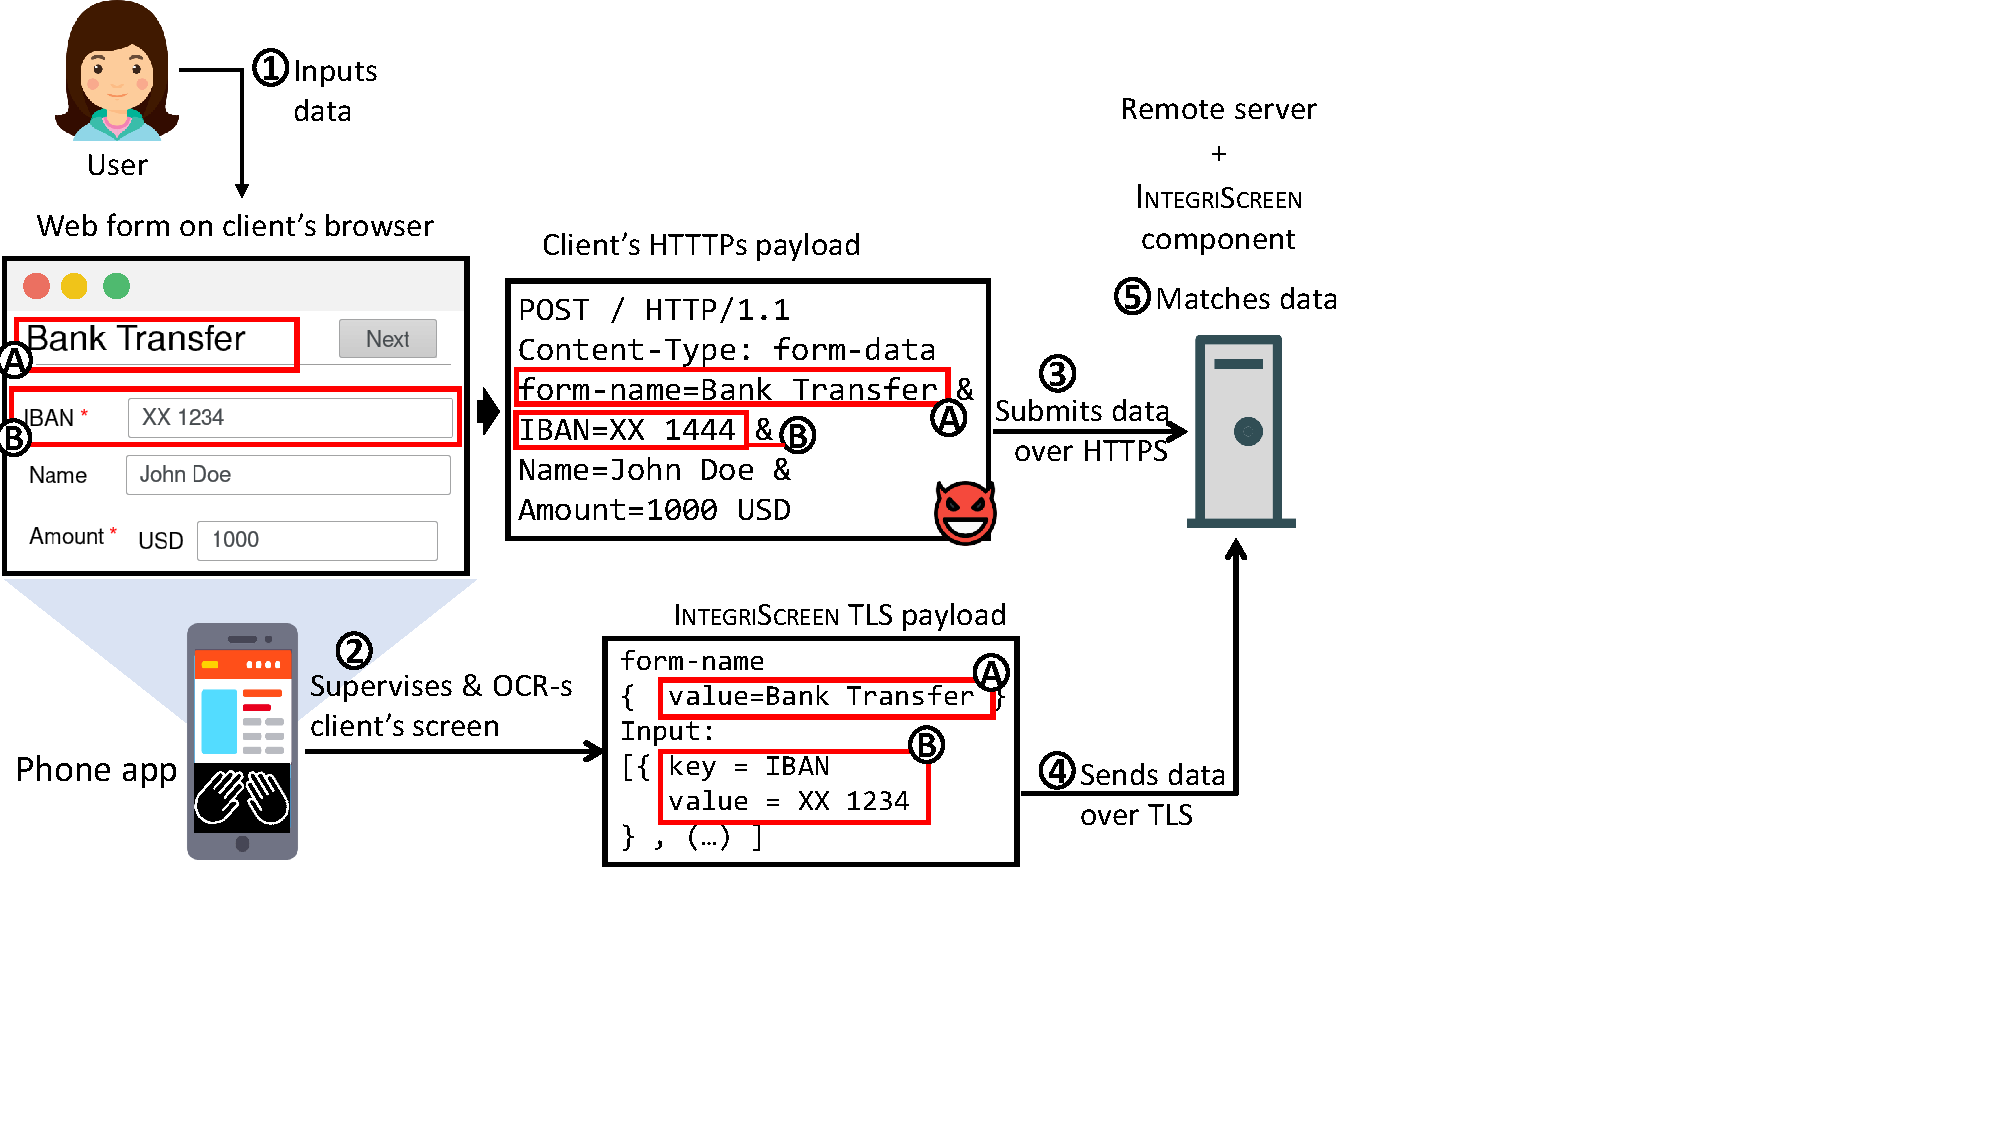
\includegraphics[trim={0 3.7cm 11.2cm 0},clip,width=\linewidth]{chapters/IntegriScreen/newImg/overview-vertical.pdf}
	\caption[System model of a visual supervision system]{\textbf{System model of a visual supervision system.} The figure shows the overall approach of the visual supervision system. The phone application continuously captures the user's screen. The phone application verifies the UI, records user input, signs the input, and sends them to the remoter server. The server receives payloads both from the browser and the phone application and checks if they match.}
	\label{integriscreen:fig:systemModel}
\end{figure}


\myparagraph{Adversary model}
We assume that the host and the network are fully compromised: the adversary can arbitrarily modify the UI elements on the screen, execute keystrokes, or simulate mouse events in the device it controls. As the adversary controls the network, he can observe, modify, or drop any network packet between the remote server and the host.
However, we assume that the smartphone is not compromised; only the legitimate user can unlock the device and run applications. The remote server is considered to be trusted. 
We assume that it is infeasible for an adversary who performs opportunistic attacks to compromise all the user devices at the same time. This is further reinforced by the fact that these second-factor devices have different hardware architecture and OS compared to the traditional host PC that the user owns. Moreover, such an attacker model is in line with the existing second-factor proposals.

The adversary's goal is to trick the remote server into accepting a request that does not correspond with the legitimate user's intended input.
Finally, we consider the privacy of user inputs and denial of service attacks to be out of the scope of this work.